\section{Dynamic Scalable State Machine Replication}
\label{sec:dssmr}

In this section, we introduce Dynamic \ssmr{} (\dssmr), discuss performance optimizations, and argue about its correctness.

\subsection{General idea}
\label{sec:generalidea}

%S-SMR divides the state variables $v$ into $k$ partitions $\ppm_1, ..., \ppm_k$, where for each $\ppm_i$, $\ppm_i \subseteq \vvm$, and each variable $v$ in $\vvm$ has to be assigned to at least one partition and define $part(v)$ as the partitions that hold $v$. Each partition $\ppm_i$ is replicated by servers in group $s_i$. For brevity, the server $s$ belongs to $\ppm_i$ with the meaning that $s \in \ssm_i$, and say that client $c$ multicasts command $C$ to partition $\ppm_i$ means that $c$ multicasts $C$ to group $\ssm_i$.
%
%To execute command $C$, the client multicasts $C$ to all partitions that hold a variable read or updated by $C$.
%Consequently, the client must be able to determine the partitions accessed by $C$, denoted by $part(C)$. If the client cannot accurately estimate which partitions are accessed by $C$, it must determine a superset of these partitions, in the worst case assuming all partitions.
%In order for clients to provide a close approximation to the command's actually accessed partitions, there is an oracle that tells the client which partitions should receive each command.



Dynamic \ssmr\ (\dssmr) defines a dynamic mapping of variables to partitions.
Each variable $v$ is mapped to partition $\ppm$, meaning that $v \in \ppm$.
Such a mapping is managed by a partitioning oracle, which is implemented as a replicated service run by group of server processes $\ssm_0$.
The oracle service allows the mapping of variables to partitions to be retrieved or changed during execution.
In more detail, \dssmr\ distinguishes five types of commands:
$access(\omega)$ is an application command that accesses (reads or writes) variables in set $\omega \subseteq \vvm$ (as described in Section~\ref{sec:background}),
$create(v)$ creates a new variable $v$ and initially maps it to a partition defined by the oracle,
$delete(v)$ removes $v$ from the service state,
% resulting in $part(v) = \emptyset$,
$move(v,\ppm_s,\ppm_d)$ moves variable $v$ from partition $\ppm_s$ to partition $\ppm_d$,
and $consult(C)$ asks the oracle which variables are accessed by command $C$, and which partition contains each of them.
The reply from the oracle to a $consult$ command is called a $prophecy$.
A prophecy usually consists of a set of tuples $\langle v, \ppm \rangle$, meaning that variable $v$ is mapped to partition $\ppm$.
The other possible values for a prophecy are $ok$ and $nok$, which mean that command can and cannot be executed, respectively (more details in Section~\ref{sec:algorithm}).
%If $v$ is not part of the service state (i.e., it was deleted or never created), the prophecy will contain~$\langle v, \emptyset \rangle$.

% explain which partitions deliver each partitioning command:
% how are access, consult, create, move and delete implemented?

%Once the oracle is in place, 
Clients can consult the oracle to know which partitions each command should be multicast to, based on which variables are accessed by the command.
If the reply received from the oracle tells the client that the command accesses a single partition, the client multicasts the command to that partition.
If the command accesses variables from multiple partitions, the client first multicasts one or more $move$ commands to the oracle and to the involved partitions, with the intent of having all variables in the same partition.
Then, the command itself is multicast to the one partition that now holds all variables accessed by the command.
If a subsequent command accesses the same variables, it will also access a single partition.
With this scheme, the access patterns of commands will shape the mapping of variables to partitions, reducing the number of multi-partition commands.

\begin{figure*}
\begin{minipage}[b]{1.0\linewidth} % A minipage that covers the whole width of the page
\centering
      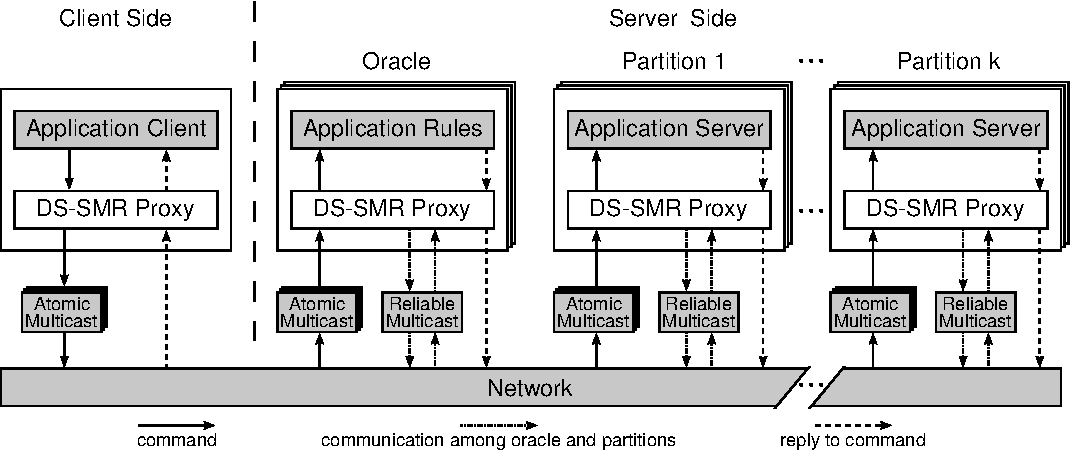
\includegraphics[width=0.8\linewidth]{figures/arch}
\end{minipage}
\caption{The architecture of \dssmrlong{}.}
\label{fig:arch}
\end{figure*}

Consulting the oracle and issuing the application command are done with separate calls to atomic multicast in \dssmr{}.
It may happen that, between those operations, the partitioning changes.
We illustrate this in Figure~\ref{fig:move_case_1}.
Commands $C_1$ and $C_2$ read variable $x$.
Since partitioning is dynamic, the client issuing the commands first consults the oracle before multicasting each command.
$C_1$ executes without the interference of other commands, so consulting the oracle and multicasting the command only once is enough for $C_1$ to be executed.
However, before $C_2$ is multicast to $\ppm_1$, another client issues a $move$ command that relocates $x$ to $\ppm_2$.
When $C_2$ is delivered at the servers of $\ppm_1$, the command is not executed, since $x$ is not available at $\ppm_1$ anymore.
A similar situation may arise when a command accesses variables from multiple partitions, as it consists of multicasting at least three commands separately: $consult$, $move$ and $access$.
The partitioning can change between the execution of any two of those commands.



%\begin{figure}[b!]
%  \includegraphics[width=\linewidth]{figures/move_case_1}
%  \caption{Consulting the oracle and issuing an application command consist of multiple calls to \amcast{}.}
%  \label{fig:move_case_1}
%\end{figure}
% \pagebreak
To solve this problem, the client multicasts the set of variables accessed along with each access command.
Upon delivery, each server checks the set of variables sent by the client.
If all variables in the set belong to the local partition, the command is executed; otherwise, a $retry$ message is sent back to the client.
When the client receives a $retry$ message, it consults the oracle again, possibly moving variables across partitions, and then reissues the access command.
To guarantee termination, if the command fails a certain number of times, the client multicasts the command to all partitions and the servers execute it as in the original \ssmr{}.

% detail create, move and delete, and explain that they are multi-partition commands, with need for signaling

% in the detailed algorithm, say that, from the pov of the client, there are no partitions

The \dssmr\ client consists of the application logic and a client proxy.
%From the point of view of the application client, there are no partitions, but only state variables to be created, accessed or deleted.
The application does not see the state variables divided into partitions.
When the application issues a command, it sends the command to the proxy and eventually receives a reply.
All commands that deal with partitioning (i.e., consulting the oracle, moving objects across partitions and retrying commands as described in the previous paragraph) are executed by the client proxy, transparently to the application.
When the client proxy multicasts a partitioning-related command to multiple partitions and the oracle, partitions and oracle exchange signals to ensure linearizability, as mentioned in Section~\ref{sec:ssmr}.
Every server and oracle process has its own \dssmr\ proxy as well.
At each server, the proxy checks whether commands can be executed and manages the exchange of data and signals between processes.
At the oracle, the service designer defines the application-dependent rules that must be followed (e.g., where each variable is created at first) and a proxy is responsible for managing the communication of the oracle with both clients and servers when executing commands.
\dssmr\ relies on a fault-tolerant multicast layer for disseminating commands across replicas and implementing reliable communication between partitions.
Replies to commands are sent directly through the network.
Figure~\ref{fig:arch} illustrates the architecture of \dssmr{}.

\subsection{Detailed algorithm}
\label{sec:algorithm}

% each proxy has only partial information

When issuing a command, the application simply forwards the command to the client proxy and waits for the reply.
Consulting the oracle and multicasting the command to different partitions is done internally by the proxy at the client.
Algorithms~\ref{alg:client_proxy}, \ref{alg:server_proxy}, and \ref{alg:oracle_proxy} describe in detail how the \dssmr\ proxy works respectively at client, server and oracle processes.
Every server proxy at a server in $\ssm_i$ has only partial knowledge of the partitioning: it knows only which variables belong to $\ppm_i$.
The oracle proxy has knowledge of every $\ppm \in \Psi$.
To maintain such a global knowledge, the oracle must \amdel{} every command that creates, moves, or deletes variables.
In order to avoid turining the oracle into a bottleneck, a caching mechamism could be applied on client to store those knoweldge as described later in Section~\ref{sec:optm}\fxnote[draft]{Add forward reference for caching}
\begin{algorithm}[h!]
\small

\begin{distribalgo}[1]

\vspace{1.0mm}

\INDENT{To issue a command $C$, the client proxy does:}

\vspace{1.0mm}

    \INDENT{\textbf{do}}
        \STATE \amcast$($oracle, $consult(C))$
        \STATE wait for $prophecy$
        \IF{$prophecy \in \{ok, nok\}$}
            \STATE $reply \leftarrow prophecy$
        \ELSE
            \STATE $C.vars \leftarrow \{v: \exists P : \langle v, P \rangle \in prophecy \}$
            \STATE $C.dests \leftarrow \{P: \exists v : \langle v, P \rangle \in prophecy \}$
            \IF{$C$ is an $access$ command and $|C.dests| > 1$}
                \STATE let $P_d$ be one of the partitions in $C.dests$
                \FOR{every $v \in C.vars$}
                    \STATE // \textit{move $v$ partition $P_d$}
                    \STATE let $P_o$ be $P : \langle v, P \rangle \in prophecy$
                    \IF{$P_o \neq P_d$}
                        \STATE $C_{move} \leftarrow move(v,P_d)$
                        \STATE $C_{move}.dests \leftarrow \{$oracle$,P_o,P_d\}$    
                        \STATE \amcast$(C_{move}.dests$, $C_{move})$
                    \ENDIF
                \ENDFOR
                \STATE $C.dests \leftarrow \{ P_s \}$
            \ENDIF
            \IF{$C$ is $create$ or $delete$}
                \STATE $C.dests \leftarrow dests \cup \{oracle\}$
            \ENDIF
            \STATE \amcast$(C.dests$, $C)$
            \STATE wait for $reply$
        \ENDIF
    \ENDINDENT
    \STATE{\textbf{while} $reply = retry$ // \textit{after $n$ retries, fall back to \ssmr}}
    \STATE return $reply$ to the application client
\ENDINDENT

\caption{\dssmr\ Client Proxy}
\label{alg:client_proxy}
\end{distribalgo}
\end{algorithm}

\textbf{The client proxy.} To execute a command $C$, the proxy first consults the oracle.
The oracle knows all state variables and which partition contains each of them.
Because of this, the oracle may already tell the client whether the command can be executed or not.
Such is the case of the $access(\omega)$ command: if there is a variable $v \in \omega$ that the command tries to read or write and $v$ does not exist, the oracle already tells the client that the command cannot be executed, by sending $nok$ as the prophecy.
A $nok$ prophecy is also returned for a $create(v)$ command when $v$ already exists.
For a $delete(v)$ command when $v$ already does not exist, an $ok$ prophecy is returned.
If the command can be executed, the client proxy receives a prophecy containing a pair $\langle v, \ppm \rangle$, for every variable $v$ created, accessed or deleted by the command.
If the prophecy regarding an $access(\omega)$ command contains multiple partitions, the client proxy chooses one of them, $\ppm_d$, and tries to move all variables in $\omega$ to $\ppm_d$.
Then, the command $C$ itself is multicast to $\ppm_d$.
As discussed in Section~\ref{sec:generalidea}, there is no guarantee that an interleave of commands will not happen, even if the client waits for the replies to the move commands.
For this reason, and to save time, the client proxy multicasts all move commands at once.
Commands that change the partitioning (i.e., create and delete) are also multicast to the oracle.
If the reply received to the command is $retry$, the procedure restarts: the proxy consults the oracle again, possibly moves variables across partitions, and multicasts $C$ to the appropriate partitions once more.
After reaching a given threshold of retries for $C$, the proxy falls back to \ssmr{}, multicasting $C$ to all partitions (and the oracle, in case $C$ is a create or delete command), which ensures the command's termination.

\begin{algorithm}[h!]
\small

\begin{distribalgo}[1]

\vspace{1.0mm}

\INDENT{To execute a command $C$, the server proxy in partition $\ppm$ does:}

    \vspace{1.0mm}
    
    \INDENT{\textbf{when} \rmdel$( \langle val, C \rangle )$}
        \STATE $rcvd\_msgs \leftarrow rcvd\_msgs \cup \{\langle val, C \rangle\}$
    \ENDINDENT

    \vspace{1.0mm}

    \INDENT{\textbf{when} \amdel$(C)$}

    \vspace{1.0mm}

        \IF{\underline{$C$ is an $access(\omega)$ command}}
            \IF{$\exists v \in \omega : v \not\in \ppm$}
                \STATE reply with $retry$
            \ELSE
                \STATE have the command executed by the application server
                \STATE send the reply to the client
            \ENDIF
        

        \vspace{1.0mm}
    
        \ELSIF{\underline{$C$ is a $move(v,\ppm_s,\ppm_d)$ command}}
            \IF{$\ppm = \ppm_s$}
                \IF{$v \in \ppm$}
                    \STATE \rmcast$(\ppm_d$,$\langle v, C \rangle)$
                    \STATE $\ppm \leftarrow \ppm \setminus \{v\}$
                \ELSE
                    \STATE \rmcast$(\ppm_d$,$\langle null, C \rangle)$
                \ENDIF
            \ELSE
                \STATE wait until $\exists val : \langle val, C \rangle \in rcvd\_msgs$
                \IF{$val \neq null$}
                    \STATE $v \leftarrow val$
                    \STATE $\ppm \leftarrow \ppm \cup \{v\}$
                \ENDIF
            \ENDIF
        
        \vspace{1.0mm}
    
        \ELSIF{\underline{$C$ is a $create(v)$ command}}
            \STATE wait until $\langle val, C \rangle \in rcvd\_msgs$
            \IF{$val = ok$}
                \STATE $\ppm \leftarrow \ppm \cup \{v\}$
%                \STATE reply with $success$
%            \ELSE
%                \STATE reply with $retry$
            \ENDIF
        
        \vspace{1.0mm}
        
        \ELSIF{\underline{$C$ is a $delete(v)$ command}}
            \IF{$v \in \ppm$}
                \STATE $\ppm \leftarrow \ppm \setminus \{v\}$
%                \STATE reply with $success$
%            \ELSE
%                \STATE reply with $retry$
            \ENDIF
        \ENDIF
    \ENDINDENT
\ENDINDENT

\caption{\dssmr\ Server Proxy}
\label{alg:server_proxy}
\end{distribalgo}
\end{algorithm}

\textbf{The server proxy.} Upon delivery, access commands are intercepted by the \dssmr\ proxy before they are executed by the application server.
In \dssmr{}, every access command is executed in a single partition.
If a server proxy in partition $\ppm$ intercepts an $access(\omega)$ command that accesses a variable $v \in \omega$ that does not belong to $\ppm$, it means that the variable is in some other partition, or it does not exist.
Either way, the client should retry with a different set of partitions, if the variable does exist.
To execute a $delete(v)$ command, the server proxy at partition $\ppm$ simply removes $v$ from partition $\ppm$, in case $v \in \ppm$.
In case $v \not\in \ppm$, it might be that the variable exists but belongs to some other partition $\ppm'$.
Since only the oracle and the servers at $\ppm'$ have this knowledge, it is the oracle who replies to delete commands.

\dssmr\ server and oracle proxies coordinate to execute commands that create or move variables.
Such coordination is done by means of \rmcast{}.
When a $create(v)$ command is delivered at $\ppm$, the server proxy waits for a message from the oracle, telling whether the variable can be created or not, to be \rmdel{}ed.
Such a message from the oracle is necessary because $v$ might not belong to $\ppm$, but it might belong to some other partition $\ppm'$ that servers of $\ppm$ have no knowledge of.
If the create command can be executed, the oracle can already reply to the client with a positive acknowledgement, saving time.
This can be done because atomic multicast guarantees that all non-faulty servers at $\ppm$ will eventually deliver and execute the command.
As for move commands, each $move(v,\ppm_s,\ppm_d)$ command consists of moving variable $v$ from a source partition $\ppm_s$ to a destination partition $\ppm_d$.
If the server's partition $\ppm$ is the source partition (i.e., $\ppm$ = $\ppm_s$), the server proxy checks whether $v$ belongs to $\ppm$.
If $v \in \ppm$, the proxy \rmcast{}s $\langle v, C \rangle$ to $\ppm_d$, so that servers at the destination partition know the most recent value of $v$; $C$ is sent along with $v$ to inform which move command that message is related to.
If $v \not\in \ppm$, a $\langle null, C \rangle$ message is \rmcast\ to $\ppm_d$, informing $\ppm_d$ that the move command cannot be executed.

\begin{algorithm}[t!]
\small

\begin{distribalgo}[1]

%\vspace{1.0mm}

	\INDENT[\textbf{Task 1}]{\colorbox{\coloralgo}{\textbf{when} \amdel$(consult(C))$}}
%		\INDENT{\textbf{case} $C$ is a $consult(C_c)$ command:}
%			\STATE $update(G_W, \omega)$
			\INDENT{\textbf{case} $C$ is a $create(v)$ command:}
				\IF[if $v$ already exists...]{$\parts(\{v\}) \neq \bot$}
					\STATE $prophecy \leftarrow nok$
					\COMMENT{...notify client}
				\ELSE[if $v$ doesn't exist...]
					\STATE $\ppm \leftarrow target(G_W, \{v\})$
					\COMMENT{...determine $v$'s partition}
					\STATE $prophecy \leftarrow (\{ \ppm, oracle \}, false)$
%					\COMMENT{prepare client's response}
				\ENDIF
			\ENDINDENT
			\INDENT{\textbf{case} $C$ is an $access(\omega)$ command:}
				\IF[if $v$ doesn't exist:]{$\exists v \in \omega : \parts(\{v\}) = \bot$}
					\STATE $prophecy \leftarrow nok$
					\COMMENT{tell the client}
				\ELSE[if all vars in $\omega$ exist]
%					\STATE $dests \leftarrow \emptyset$
%					\FOR{each $v \in \omega$}
%						\STATE $dests \leftarrow dests \cup partition(v)$
%					\ENDFOR
					\STATE $dests \leftarrow \parts(\omega)$
					\COMMENT{get all partition involved}
					\IF[if only one partition:]{$|dests| = 1$}
						\STATE $prophecy \leftarrow (dests,false)$
%						\COMMENT{tell client which partition}
					\ELSE[if multiple partitions involved]
						\STATE $\ppm_d \leftarrow target(G_W, \omega)$
						\COMMENT{$\ppm_d$ will store all vars in $\omega$}
						\STATE $alldest \leftarrow \{oracle\} \cup dests$
						\COMMENT{move $v$ from $\ppm_s$...}
						\STATE \amcast$(alldest, move(\omega,dests,\ppm_d))$
						\COMMENT{...to $\ppm_d$}						
%						\FOR[for each involved var $v$]{each $v \in \omega$}
%							\STATE $\ppm_s \leftarrow \parts(\{v\})$
%							\COMMENT{$\ppm_s$ is $v$'s current partition}
%							\IF[if $v$ not in $\ppm_d$:]{$\ppm_s \neq \ppm_d$}
%								\STATE $aux \leftarrow \{oracle,\ppm_s,\ppm_d\}$
%								\COMMENT{move $v$ from $\ppm_s$...}
%								\STATE \amcast$(aux$, $move(v,\ppm_s,\ppm_d))$
%								\COMMENT{...to $\ppm_d$}
%							\ENDIF 
%						\ENDFOR
						\STATE $prophecy \leftarrow (\{\ppm_d\},true)$
					\ENDIF 
				\ENDIF
			\ENDINDENT
			\STATE send $prophecy$ to the client
%			\INDENT{\textbf{case} $C_c$ is a $delete(v)$ command:}
%				\IF{$partition(v) = \bot$}
%					\STATE $prophecy \leftarrow ok$
%				\ELSE
%					\STATE $prophecy \leftarrow (\{ \ppm : v \in \ppm, oracle \}, -)$
%				\ENDIF
%			\ENDINDENT
%		\ENDINDENT
	\ENDINDENT
	\vspace{1.0mm}

	\INDENT[\textbf{Task 2}]{\colorbox{\coloralgo}{\textbf{when} \amdel$(create(v))$}}
%	\INDENT{\textbf{case} $C$ is a $create(v)$ command:}
		\STATE let $\ppm_c \in C.dests \setminus \{oracle\}$
		\COMMENT{var created in $\ppm_c$}
		\STATE \rmcast$(\ppm_c, \langle signal, C \rangle )$
		\COMMENT{exchange signal to...}
		\STATE wait until $\langle signal, C \rangle \in rcvd\_msgs$
		\COMMENT{...coordinate partitions}
		\STATE $\ppm_c \leftarrow \ppm_c \cup      \{v\}$
                \STATE send $ok$ to the client
	\ENDINDENT

	\vspace{1.0mm}
	\INDENT[\textbf{Task 3}]{\colorbox{\coloralgo}{\textbf{when} \amdel$(move(\omega,dests,\ppm_d))$}}
%        \INDENT{\textbf{case} $C$ is a $move(v,\ppm_s,\ppm_d)$ command:}
                \STATE \textbf{for} each $\ppm_s \in dests$ \textbf{do} $\ppm_s \leftarrow \ppm_s \setminus \omega$
                \COMMENT{update partitions...}
                \STATE $\ppm_d \leftarrow \ppm_d \cup \omega$
                \COMMENT{...and add new variables}
                \STATE send $ok$ to the client
	\ENDINDENT

        \vspace{1.0mm}
    
	\INDENT[\textbf{Task 4}]{\colorbox{\coloralgo}{\textbf{when} \rmdel$( \langle val, C \rangle )$}}
		\STATE $rcvd\_msgs \leftarrow rcvd\_msgs \cup \{\langle val, C \rangle\}$
	\ENDINDENT
	
	\vspace{1.0mm}
	\INDENT{\colorbox{\coloralgo}{\textbf{function} \parts$(vars)$}}
		\STATE $aux \leftarrow \{ \ppm : \exists v \in vars \cap \ppm \}$
		\STATE return $aux$
	\ENDINDENT
	
%	\vspace{1.0mm}
	\rule{83mm}{0.4pt}
%	\vspace{0.1mm}

	\INDENT[\textbf{Task 5}]{\colorbox{\coloralgo}{\textbf{when} \amdel$(hint(V_h,E_h))$}}
		\STATE update $G_W$ with $(V_h,E_h)$
%		\STATE send $ok$ to the client
	\ENDINDENT
	
	\vspace{1.0mm}
    
	\INDENT[\textbf{Task 6}]{\colorbox{\coloralgo}{\textbf{periodically} do}}
		\STATE compute ideal partition $\ip_1, ..., \ip_m$ from $G_W$
	\ENDINDENT
	
	\vspace{1.0mm}
    
	\INDENT{\colorbox{\coloralgo}{\textbf{function} target$(vars)$}}
		\STATE $\ppm \leftarrow$ compute destination partition for $vars$ from\\ \hspace{8mm}current $\ppm_1, ..., \ppm_m$ and ideal $\ip_1, ..., \ip_m$ partitionings
		\STATE return $\ppm$
	\ENDINDENT	
	
%	\vspace{1.0mm}
%        
%	\INDENT{\textbf{case} $C$ is a $delete(v)$ command:}
%		\STATE let $\ppm_d$ be $\ppm : \{\ppm\} = C.dests \setminus \{$oracle$\}$
%		\STATE $\ppm_c \leftarrow \ppm_c \setminus      \{v\}$
%		\STATE \rmcast$(\ppm_c, \langle ok, C \rangle )$
%			\STATE wait until $\exists val : \langle val, C \rangle \in rcvd\_msgs$
%	\ENDINDENT

%\ENDINDENT

\caption{Oracle}
\label{alg:oracle_proxy}
\end{distribalgo}
\end{algorithm}

\textbf{The oracle proxy.} One of the purposes of the oracle proxy is to make prophecies regarding the location of state variables.
Such prophecies are used by client proxies to multicast commands to the right partitions.
A prophecy regarding an $access(\omega)$ command contains, for each $v \in \omega$, a pair $\langle v, \ppm \rangle$, meaning that $v \in \ppm$.
If any of the variables in $\omega$ does not exist, the prophecy already tells the client that the command cannot be executed (with a $nok$ value).
For a $create(v)$ command, the prophecy tells where $v$ should be created, based on rules defined by the application, if $v$ does not exist.
If $v$ already exists, the prophecy will contain $nok$, so that the client knows that the create command cannot be executed.
The prophecy regarding a $delete(v)$ command contains the partition that contains $v$, or $ok$, in case $v$ was already deleted or never~existed.

Besides dispensing prophecies, the oracle is responsible for executing create, move, and delete commands, coordinating with server proxies when necessary, and replying directly to clients in some cases.
For each $move(v,\ppm_s,\ppm_d)$ command, the oracle checks whether $v$ in fact belongs to the source partition $\ppm_s$.
If that is the case, the command is executed, moving $v$ to $\ppm_d$.
Each $create(v)$ command is multicast to the oracle and to a partition $\ppm$.
If $v$ already exists, the oracle tells $\ppm$ that the command cannot be executed, by \rmcast{}ing $nok$ to $\ppm$.
The oracle also sends $nok$ to the client as reply, meaning that $v$ already exists.
If $v$ does not exist, the oracle tells $\ppm$ that the command can be executed, by \rmcast{}ing $ok$ to $\ppm$.
It also tells the client that the command succeeded with an $ok$ reply.
Finally, each $delete(v)$ command is multicast to the oracle and to a partition $\ppm$, where the client proxy assumed $v$ to be located.
If $v$ belongs to $\ppm$, or $v$ does not exist, the oracle tells the client that the delete command succeeded.
Otherwise, that is, if $v$ exists, but $delete(v)$ was multicast to the wrong partition, the oracle tells the client to retry.



\subsection{Performance optimizations}
\label{sec:optm}

In this section, we introduce two optimizations for \dssmr{}: caching and load balancing.

\textbf{Caching.} In Algorithm~\ref{alg:client_proxy}, for every command issued by the client, the proxy consults the oracle.
If every command passes by the oracle, the system is unlikely to scale, as the oracle is prone to becoming a bottleneck.
To provide a scalable solution, each client proxy has a local cache of the partitioning information.
Before multicasting an application command $C$ to be executed, the client proxy checks whether the cache has information about every variable concerned by $C$.
If the cache does have such a knowledge, the oracle is not consulted and the information contained in the cache is used instead.
If the reply to $C$ is $retry$, the oracle is consulted and the returned prophecy is used to update the client proxy's cache.
Algorithm~\ref{alg:client_proxy} is followed from the second attempt to execute $C$ on.
The cache is a local service that follows an algorithm similar to that of the oracle, except it responds only to $consult(C)$ commands and, in situations where the oracle would return $ok$ or $nok$, the cache tells the client proxy to consult the actual oracle.



%\begin{figure}
%  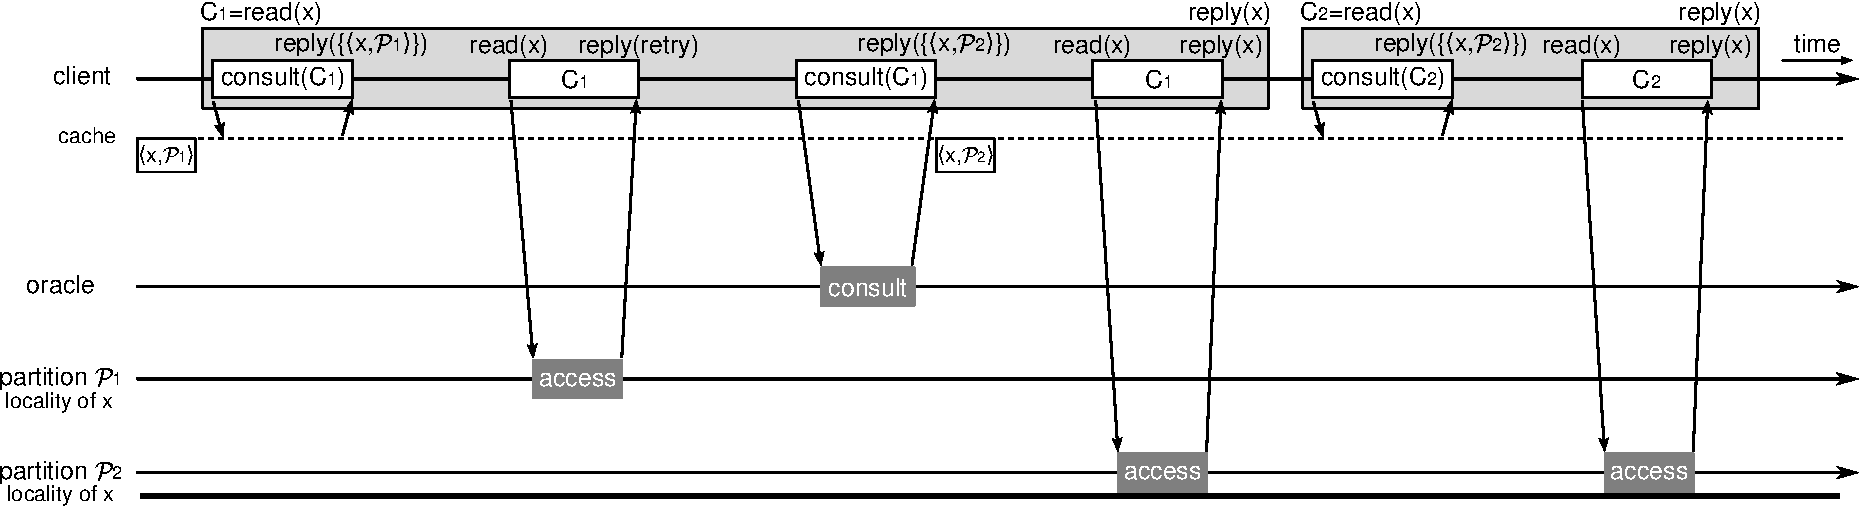
\includegraphics[width=\linewidth]{figures/cache_retry}
%  \caption{A cache is used by each client to avoid consulting the oracle.}
%  \label{fig:cache_retry}
%\end{figure}

Naturally, the cached partitioning information held by the client proxy may be out of date.
On the one hand, this may lead a command to be multicast to the wrong set of partitions, which will probably incur in the client proxy having to retry executing the command.
For instance, in Figure~\ref{fig:cache_retry} the client has an out-of-date cache, incurring in a new consultation to the oracle when executing $C_3$.
On the other hand, the client proxy may already have to retry commands, even if the oracle is always consulted first, as shown in Figure~\ref{fig:move_case_1}.
If most commands are executed without consulting the oracle, as in the case of $C_4$ in Figure~\ref{fig:cache_retry}, we avoid turning the oracle into a bottleneck.
Moreover, such a cache can be updated ahead of time, not having to wait for an actual application command to be issued to only then consult the oracle.
This way, the client proxy can keep a cache of partitioning information of variables that the proxy deems likely to be accessed in the future.

\textbf{Load balancing}. When moving variables, the client proxies may try to distribute them in a way that balances the workload among partitions.
This way, the system is more likely to scale throughput with the number of server groups.
One way of balancing load is by having roughly the same number of state variables in every partition.
This can be implemented by having client proxies choosing randomly the partition that will receive all variables concerned by each command (at line~\ref                {algline:client:partition} of Algorithm~\ref{alg:client_proxy}).
Besides improving performance, balancing the load among partitions prevents the system from degenerating into a single-partition system, with all variables being moved to the same place as commands are executed.


%Algorithm 1 can be optimized in many ways. In this section, we briefly mention some of these optimizations and then detail caching.

%Client can have a cache copy of the variable location on local. Thus when client issues command $C$, it does not need to query Oracle, instead it send a message direct to the associated partition based on its knowledge from cache. There are possibilities that client cache is invalid because of move command other client issued, thus the partition just need to return a response indicates invalid location. Then the client can retry the command by starting query from Oracle this time to get the updated location of state variable. 

%\begin{figure*}
%\begin{minipage}[b]{1\linewidth} % A minipage that covers the whole width of the page
%\centering
%      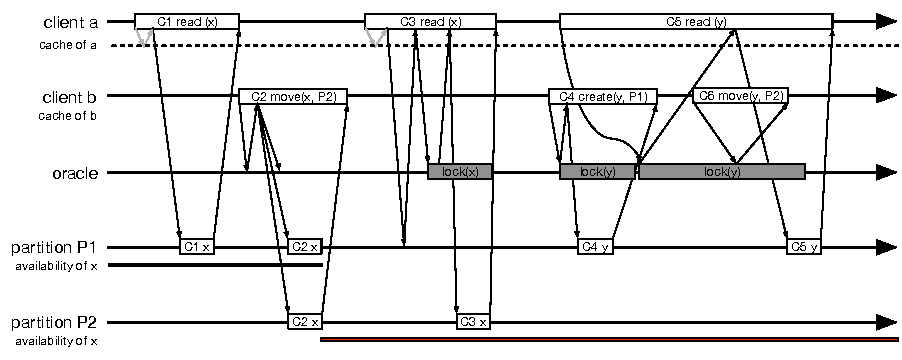
\includegraphics[width=0.85\linewidth]{figures/cache}
%\end{minipage}
%\caption{Execution flow of DS-SMR with oracle caching on client}
%\label{fig:cache}
%\end{figure*}

\begin{figure*}
\begin{minipage}[b]{1\linewidth} % A minipage that covers the whole width of the page
\centering
      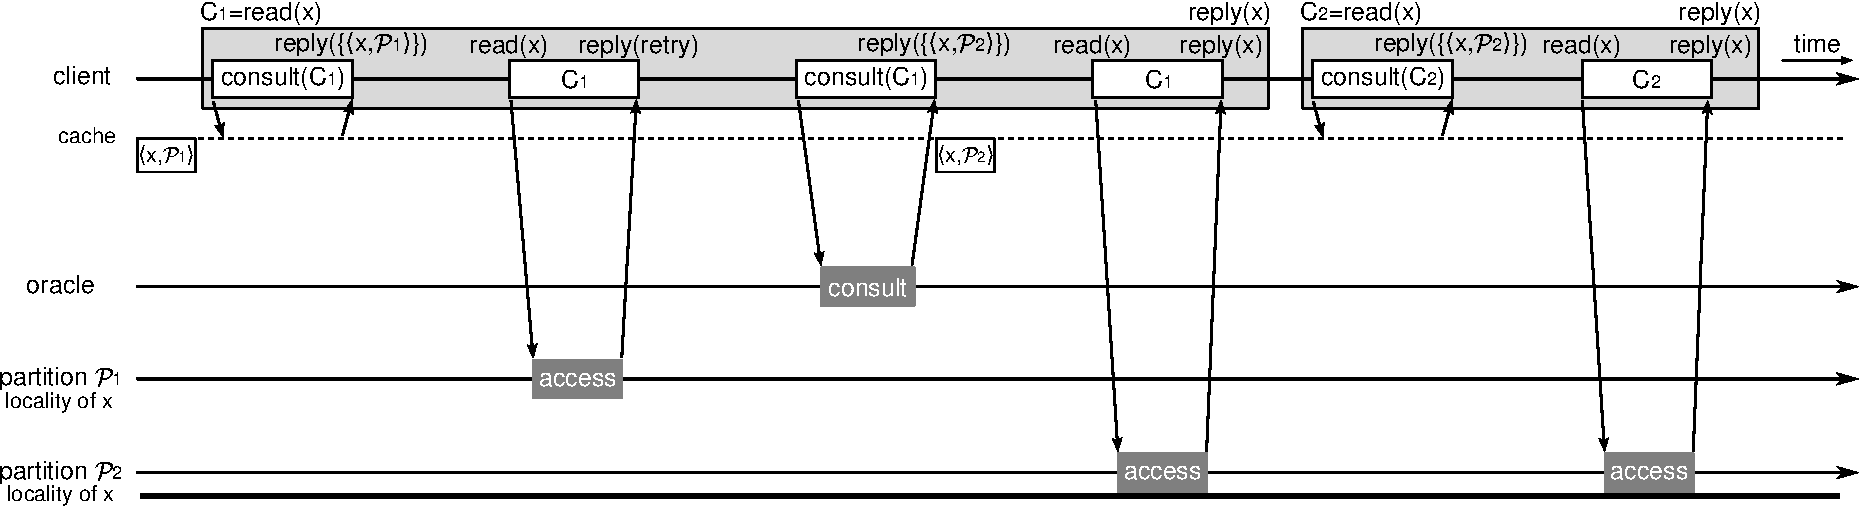
\includegraphics[width=1.0\linewidth]{figures/cache_retry}
\end{minipage}
\caption{Each client proxy in \dssmr\ maintains a cache in order to avoid  consulting the oracle. White boxes represent actions of the client proxy.}
\label{fig:cache_retry}
\end{figure*}

\subsection{Correctness}
\label{sec:correctness}

In this section, we argue that \dssmr\ ensures termination and linearizability.
By ensuring termination, we mean that for every command $C$ issued by a correct client, a reply to $C$ different than $retry$ is eventually received by the client.
This assumes that at least one oracle process is correct and that every partition has at least one correct server.
Given these constraints, the only thing that could prevent a command from terminating would be an execution that forced the client proxy to keep retrying a command.
This problem is trivially solved by falling back to \ssmr\ after a predefined number of retries: at a certain point, the client proxy multicast the command to all server and oracle processes, which execute the command as in \ssmr{}, i.e., with coordination among all partitions and the oracle.

As for linearizability, we argue that, if every command in execution \ex\ of \dssmr\ is delivered by atomic multicast and is \emph{execution atomic} (as defined in~\cite{bezerra2014ssmr}), then \ex\ is linearizable.
We denote the order given by atomic multicast by relation $\prec$.
Given any two messages $m_1$ and $m_2$, ``$m_1 \prec m_2$'' means that there exists a process that delivers both messages and $m_1$ is delivered before $m_2$, or there is some message $m'$ such that $m_1 \prec m'$ and $m' \prec m_2$, which can be written as \mbox{$m_1 \prec m' \prec m_2$}.\fxnote[draft]{use the phrase \"there exists a process that\" }
Also, for the purposes of this proof, we consider the oracle to be a partition, as it also \amdel{}s and executes application commands.

Suppose, by means of contradiction, that there exist two commands $x$ and $y$, where $x$ finishes before $y$ starts, but $y \prec x$ in the execution.
There are two possibilities to be considered: (i) $x$ and $y$ are delivered by the same process $p$, or (ii) no process delivers both $x$ and $y$.

In case (i), at least one process $p$ delivers both $x$ and $y$.
As $x$ finishes before $y$ starts, then $p$ delivers $x$, then $y$. From the properties of atomic multicast, and since each partition is mapped to a multicast group, no process delivers $y$, then $x$.
Therefore, we reach a contradiction in this case.

In case (ii), if there were no other commands in \ex, then the execution of $x$ and $y$ could be done in any order, which would contradict the supposition that $y \prec x$.
Therefore, there are commands $z_1, ..., z_n$ with atomic order $y \prec z_1 \prec \cdots \prec z_n \prec x$, where some process $p_0$ (of partition $\ppm_0$) delivers $y$, then $z_1$; some process $p_1 \in \ppm_1$ delivers $z_1$, then $z_2$, and so on: process $p_i \in \ppm_i$ delivers $z_{i}$, then $z_{i+1}$, where $1 \leq i < n$.
Finally, process $p_n \in \ppm_n$ delivers $z_n$, then $x$.

Let $z_0 = y$ and let $atomic(i)$ be the following predicate:
``For every process $p_i \in \ppm_i$, $p_i$ finishes executing $z_i$ only after some $p_0 \in \ppm_0$ started executing $z_0$.''
We now claim that $atomic(i)$ is true for every $i$, where $0 \leq i \leq n$.
We prove our claim by induction.

%\begin{itemize}

%\item
\emph{Basis ($i=0$)}: $atomic(0)$ is obviously true, as $p_0$ can only finish executing $z_0$ after starting executing it.

%\item
\emph{Induction step}: If $atomic(i)$, then $atomic(i+1)$.
\\
Proof: Command $z_{i+1}$ is multicast to both $\ppm_i$ and $\ppm_{i+1}$. Since $z_{i+1}$ is execution atomic, before any $p_{i+1} \in \ppm_{i+1}$ finishes executing $z_{i+1}$, some $p_i \in \ppm_i$ starts executing $z_{i+1}$.
Since $z_i \prec z_{i+1}$, every $p_i \in \ppm_i$ start executing $z_{i+1}$ only after finishing the execution of $z_i$.
As $atomic(i)$ is true, this will only happen after some $p_0 \in \ppm_0$ started executing $z_0$.

%\end{itemize}

As $z_n \prec x$, for every $p_n \in \ppm_n$, $p_n$ executes command $x$ only after the execution of $z_n$ at $p_n$ finishes.
From the above claim, this happens only after some $p_0 \in \ppm_0$ starts executing $y$.
This means that $y$ ($z_0$) was issued by a client before any client received a response for $x$,
which contradicts the assumption that $x$ precedes $y$ in real-time, i.e., that command $y$ was issued after the reply for command $x$ was received.